% !TeX root = tcolorbox.tex
% include file of tcolorbox.tex (manual of the LaTeX package tcolorbox)
\clearpage
\section{Macros for Box Creation}

\begin{docEnvironment}{tcolorbox}{\oarg{options}}
  This is the main environment to create an accentuated colored text box with
  rounded corners and, optionally, two parts. The appearance of this box
  is controlled by numerous options.
  In the most simple case the source code

\begin{dispListing}
\begin{tcolorbox}
This is a \textbf{tcolorbox}.
\end{tcolorbox}
\end{dispListing}

creates the following compiled text box:
\begin{tcolorbox}
This is a \textbf{tcolorbox}.
\end{tcolorbox}

The text content of the box can be divided
in an upper and a lower part
by the command \refCom{tcblower}. Visually, both parts are separated by a line.
For example:

\begin{dispListing}
\begin{tcolorbox}
This is another \textbf{tcolorbox}.
\tcblower
Here, you see the lower part of the box.
\end{tcolorbox}
\end{dispListing}

This code gives the following box:
\begin{tcolorbox}
This is another \textbf{tcolorbox}.
\tcblower
Here, you see the lower part of the box.
\end{tcolorbox}

The \meta{options} control the appearance and several functions of the boxes,
see section \ref{sec:optkeys} for the complete list.
A quick example is given here:

\begin{dispExample}
\begin{tcolorbox}[colback=red!5!white,colframe=red!75!black,title=My nice heading]
This is another \textbf{tcolorbox}.
\tcblower
Here, you see the lower part of the box.
\end{tcolorbox}
\end{dispExample}
\end{docEnvironment}


\begin{docCommand}{tcblower}{}
  Used inside \refEnv{tcolorbox} to separate the upper box part from
  the optional lower box part. The upper and the lower part are treated
  as separate functional units. If you only want to draw a line, see
  \refCom{tcbline}.
\end{docCommand}


\clearpage
\begin{docCommand}{tcbset}{\marg{options}}
  Sets options for every following \refEnv{tcolorbox} inside the current \TeX\ group.
  By default, this does not apply to nested boxes, see
  Section \ref{subsec:everybox} from page \pageref{subsec:everybox}.\par
  For example, the colors of the boxes may be defined for the whole document by this:
\begin{dispListing}
\tcbset{colback=red!5!white,colframe=red!75!black}
\end{dispListing}
\end{docCommand}


\begin{docCommand}{tcbox}{\oarg{options}\marg{box content}}
  Creates a colored box which is fitted to the width of the given
  \meta{box content}. In principal, most \meta{options} for a \refEnv{tcolorbox}
  can be used for |\tcbox| with some restrictions. A |\tcbox| cannot have
  a lower part and cannot be broken.

\begin{dispExample}
\tcbset{colframe=blue!50!black,colback=white,colupper=red!50!black,
        fonttitle=\bfseries,nobeforeafter,center title}

Text \tcbox[tcbox raise base]{Hello World}\hfill
%
\tcbox[left=0mm,right=0mm,top=0mm,bottom=0mm,boxsep=0mm,
  toptitle=0.5mm,bottomtitle=0.5mm,title=My table]{%
  \arrayrulecolor{blue!50!black}\renewcommand{\arraystretch}{1.2}%
  \begin{tabular}{r|c|l}
  One   & Two    & Three \\\hline\hline
  Men   & Mice   & Lions \\\hline
  Upper & Middle & Lower
  \end{tabular}}\hfill
%
\tcbox[colback=blue!85!black,
  left=0mm,right=0mm,top=0mm,bottom=0mm,boxsep=1mm,arc=0mm,boxrule=0.5pt,
  title=My picture]{%
  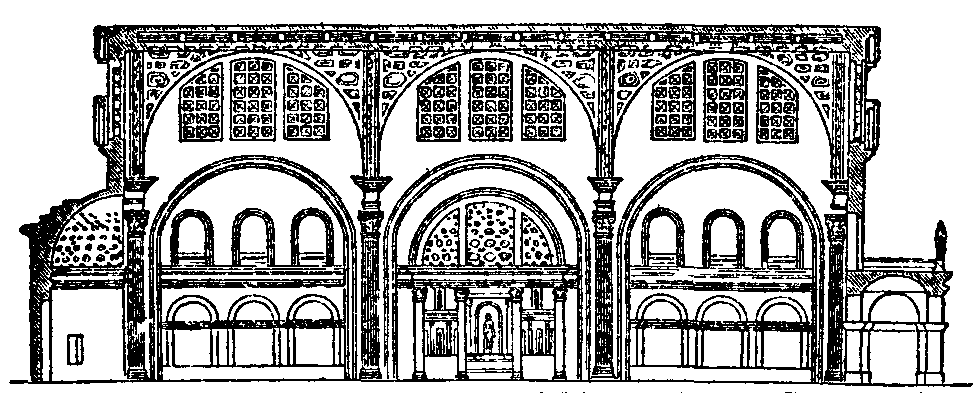
\includegraphics[width=5cm]{Basilica_5.png}}
\end{dispExample}
\end{docCommand}

\clearpage
\begin{docCommand}{newtcolorbox}{\oarg{init options}\marg{name}\oarg{number}\oarg{default}\marg{options}}
  Creates a new environment \meta{name} based on \refEnv{tcolorbox}.
  Basically, |\newtcolorbox| operates like |\newenvironment|. This means,
  the new environment \meta{name} optionally takes \meta{number} arguments, where
  \meta{default} is the default value for the optional first argument.
  The \meta{options} are given to the underlying |tcolorbox|.
  Note that \refKey{/tcb/savedelimiter} is set to the given \meta{name}
  automatically.
  The \meta{init options} allow to set up automatic numbering,
  see Section \ref{sec:initkeys} from page \pageref{sec:initkeys}.
\begin{dispExample*}{sbs,lefthand ratio=0.6}
\newtcolorbox{mybox}{colback=red!5!white,
  colframe=red!75!black}

\begin{mybox}
This is my own box.
\end{mybox}
\end{dispExample*}

\begin{dispExample*}{sbs,lefthand ratio=0.6}
\newtcolorbox{mybox}[1]{colback=red!5!white,
  colframe=red!75!black,fonttitle=\bfseries,
  title=#1}

\begin{mybox}{Hello there}
This is my own box with a mandatory title.
\end{mybox}
\end{dispExample*}

\begin{dispExample*}{sbs,lefthand ratio=0.6}
\newtcolorbox{mybox}[2][]{colback=red!5!white,
  colframe=red!75!black,fonttitle=\bfseries,
  title=#2,#1}

\begin{mybox}[colback=yellow]{Hello there}
This is my own box with a mandatory title
and options.
\end{mybox}
\end{dispExample*}

\inputpreamblelisting{A}

\begin{dispExample*}{sbs,lefthand ratio=0.6}
\begin{pabox}[colback=yellow]{Hello there}
This is my own box with a mandatory
numbered title and options.
\end{pabox}
\end{dispExample*}
\end{docCommand}


\clearpage
\begin{docCommand}{newtcbox}{\oarg{init options}\marg{\texttt{\textbackslash}name}\oarg{number}\oarg{default}\marg{options}}
  Creates a new macro \meta{\texttt{\textbackslash}name} based on \refCom{tcbox}.
  Basically, |\newtcbox| operates like |\newcommand|.
  The new macro \meta{\texttt{\textbackslash}name} optionally takes \meta{number}$+1$ arguments, where
  \meta{default} is the default value for the optional first argument.
  The \meta{options} are given to the underlying |tcbox|.
  The \meta{init options} allow to set up automatic numbering,
  see Section \ref{sec:initkeys} from page \pageref{sec:initkeys}.
\begin{dispExample*}{sbs,lefthand ratio=0.6}
\newtcbox{\mybox}{colback=red!5!white,
  colframe=red!75!black}

\mybox{This is my own box.}
\end{dispExample*}

\begin{dispExample*}{sbs,lefthand ratio=0.6}
\newtcbox{\mybox}[1]{colback=red!5!white,
  colframe=red!75!black,fonttitle=\bfseries,
  title=#1}

\mybox{Hello there}{This is my own box.}
\end{dispExample*}

\begin{dispExample*}{sbs,lefthand ratio=0.6}
\newtcbox{\mybox}[2][]{colback=red!5!white,
  colframe=red!75!black,fonttitle=\bfseries,
  title=#2,#1}

\mybox[colback=yellow]{Hello there}%
  {This is my own box.}
\end{dispExample*}

\inputpreamblelisting{B}

\begin{dispExample*}{sbs,lefthand ratio=0.6}
\pbbox[colback=yellow]{Hello there}%
  {This is my own box.}
\end{dispExample*}

\end{docCommand}



